\documentclass[12pt,a4paper,dvipdfmx]{jsarticle}
%%% PACKAGES
\usepackage{graphicx} % support the \includegraphics command and options
\usepackage{framed}
\setlength\FrameSep{0.5em}
\setlength\OuterFrameSep{\partopsep}
\usepackage{bigints}
\usepackage{textpos}
\usepackage{color,soul}
\usepackage{wrapfig}
\usepackage{mathtools}
\usepackage[all,cmtip]{xy}
\usepackage{mystyle}
\usepackage{lpic}
\usepackage{etoolbox}
\usepackage{comment}
\usepackage[normalem]{ulem}
\usepackage{setspace}
\usepackage{booktabs} % for much better looking tables
\usepackage{array} % for better arrays (eg matrices) in maths
\usepackage{paralist} % very flexible & customisable lists (eg. enumerate/itemize, etc.)
\usepackage{verbatim} % adds environment for commenting out blocks of text & for better verbatim
\usepackage{subfig} % make it possible to include more than one captioned figure/table in a single float
\usepackage{amssymb}
\usepackage{amsfonts}
\usepackage{amsmath}
\usepackage{amssymb}
\usepackage{amsfonts}
\usepackage{amsmath,amsthm}
\usepackage{amssymb,amssymb,amsthm,lmodern}
\usepackage[driver=dvipdfm,truedimen,top=3truecm,bottom=3truecm,left=2.5truecm,right=2.5truecm]{geometry}
\usepackage{xcolor}
\usepackage[dvipdfm,colorlinks=true,linkcolor=blue]{hyperref}
\usepackage{tikz}
\usetikzlibrary{shapes,arrows,patterns}
\usepackage[inline]{showlabels}
\usepackage{blindtext}
\usepackage{titlefoot}

\numberwithin{equation}{section}

\newcommand{\myre}[1]{\tmop{Re} #1}
	\newcommand{\bolds}{\mathbf{s}}
\newcommand{\mysbo}{A:\pi\kern-0.1cm\mid_{G'}\xrightarrow{G'}\tau}
\newcommand{\myrelationdiagram}[5]{
	\vspace{1em}
		\centerline{
		\xymatrix{
			\framebox{\mbox{#1}}\ar@{=>}[rd]^{\begin{array}[]{c}
				#2
			\end{array}}&&\framebox{\mbox{#4}}\ar@{=>}[ld]_{\begin{array}[]{c}
			#3
	\end{array}}\\
			&
			\framebox{\mbox{#5}}
			&
		}}
	\vspace{1em}
	}
\newenvironment{proof*}[1]{\noindent\textbf{#1\ }}{\hspace*{\fill}\medskip}
\newcommand{\myrelationdiagramBigSix}[6]{
			\begin{samepage}
				\vspace{1em}
		\centerline{
		\xymatrixcolsep{#6cm}
		\xymatrix{
			\framebox{\mbox{#1}}\ar@{=>}[rd]^{\begin{array}[]{c}
				#2
			\end{array}}&&&&\framebox{\mbox{#4}}\ar@{=>}[ld]_{\kern-1.5cm\begin{array}[]{c}
			#3
	\end{array}}\\
			&&&&
		}}
		\nopagebreak
		\framebox{\mbox{#5}}
				\vspace{1em}
			\end{samepage}
	}
\newcommand{\myrelationdiagramBigCenterSix}[6]{
			\begin{samepage}
				\vspace{1em}
		\centerline{
		\xymatrixcolsep{#6cm}
		\xymatrix{
			\framebox{\mbox{#1}}\ar@{=>}[rd]^{\begin{array}[]{c}
				#2
			\end{array}}&&&&\framebox{\mbox{#4}}\ar@{=>}[ld]_{\kern-1.5cm\begin{array}[]{c}
			#3
	\end{array}}\\
			&&&&
		}}
		\nopagebreak
		\centerline{
			\framebox{\mbox{#5}}}
				\vspace{1em}
			\end{samepage}
	}
\newcommand{\myrelationdiagramBigCenter}[5]{
			\begin{samepage}
				\vspace{1em}
		\centerline{
		\xymatrixcolsep{2.5cm}
		\xymatrix{
			\framebox{\mbox{#1}}\ar@{=>}[rd]^{\begin{array}[]{c}
				#2
			\end{array}}&&&&\framebox{\mbox{#4}}\ar@{=>}[ld]_{\kern-1.5cm\begin{array}[]{c}
			#3
	\end{array}}\\
			&&&&
		}}
		\nopagebreak
		\centerline{
			\framebox{\mbox{#5}}}
				\vspace{1em}
			\end{samepage}
	}
\newcommand{\myrelationdiagramBig}[5]{
			\begin{samepage}
				\vspace{1em}
		\centerline{
		\xymatrixcolsep{2.5cm}
		\xymatrix{
			\framebox{\mbox{#1}}\ar@{=>}[rd]^{\begin{array}[]{c}
				#2
			\end{array}}&&&&\framebox{\mbox{#4}}\ar@{=>}[ld]_{\kern-1.5cm\begin{array}[]{c}
			#3
	\end{array}}\\
			&&&&
		}}
		\nopagebreak
		\framebox{\mbox{#5}}
				\vspace{1em}
			\end{samepage}
	}

\newcommand{\red}[1]{{\color[rgb]{0.6,0,0}#1}}
	\definecolor{Blue}{rgb}{0,0.0,1}
	\definecolor{Red}{rgb}{1,0.0,0}

\newcommand*\mytextcircled[1]{\tikz[baseline=(char.base)]{
	\node[shape=circle,draw,inner sep=1.8pt] (char) {\scalebox{0.8}{\kern-0.05cm #1}};}}
\newcommand{\mybigplus}{\scalebox{2.0}{$+$}}
\renewcommand{\implies}{\Rightarrow}
\newcommand{\mypgf}{{\mbox{ガンマ関数の積}}}
\newcommand{\Sol}{\mathcal{S}\mbox{ol}}
\newcommand{\Ind}{\mbox{\normalfont Ind}}
\newcommand{\D}{\mathcal{D}}
\newcommand{\A}{\mathcal{A}}
\newcommand{\Co}{\mathbb{C}}
\newcommand{\X}{\mathbb{X}}
\renewcommand{\setminus}{\backslash}
\newcommand{\nin}{\not\in}
\newcommand{\tmop}[1]{\ensuremath{\operatorname{#1}}}
\newcommand{\tmtextbf}[1]{{\bfseries{#1}}}
\newcommand{\tmtextit}[1]{{\itshape{#1}}}
\newcommand{\mss}{//}
\newcommand{\mbb}{\backslash\backslash}
\newcommand{\mmm}{\mid\mid}
\catcode`\<=\active \def<{
\fontencoding{T1}\selectfont\symbol{60}\fontencoding{\encodingdefault}}
\catcode`\>=\active \def>{
\fontencoding{T1}\selectfont\symbol{62}\fontencoding{\encodingdefault}}
\newcommand{\assign}{:=}
\newcommand{\comma}{{,}}
\newcommand{\um}{-}
\newcommand{\sol}{\mathcal{S}ol(\R^{p,q};\lambda,\nu)}
\newcommand{\Op}{\mbox{\normalfont Op}}
\newcommand{\Res}{\operatorname{Res}\displaylimits}
\newcommand{\OpR}{\mbox{\it R}}

%%%%%%%%%%%%%%%%%%%%%%%%%%%%%%%%%%%%%%%%%%%%%%%%%%%%
\makeatletter
\def\@author@list{}
\renewcommand{\author}[4]{%
  \ifx\@author@list\@empty\else\g@addto@macro\@author@list{\medskip}\fi
  \g@addto@macro\@author@list{\noindent #2\quad#1\par\noindent #3\par\noindent #4\par}%
}
\def\@maketitle{%
  \begin{center}
  {\LARGE \@title}\par
  \vskip 1.5em
  {\large\@author@list}%
  \end{center}
  \par\vskip 1.5em
}
\let\original@proof=\proof
\let\original@endproof=\endproof
\def\proof{\@ifnextchar[{\proof@}{\proof@[\proofname]}}
\def\proof@[#1]{%
  \labelsep=1zw
  \original@proof[{\headfont #1\inhibitglue}\nopunct]
}
\makeatother
\newtheoremstyle{jplain}{}{}{\normalfont}{}{\headfont}{}{1zw}{\thmname{#1}\thmnumber{\ #2}.\thmnote{(#3)}}
\theoremstyle{jplain}
\renewcommand{\proofname}{証明}
% 概要の見出しを英語に
\renewcommand{\abstractname}{Abstract}
%%%%%%%%%%%%%%%%%%%%%%%%%%%%%%%%%%%%%%%%%%%%%%%%%%%%

% 定理環境の定義
\newtheorem{thm}{定理}[section]
\newtheorem{lem}[thm]{補題}
\newtheorem*{lemma*}{補題}
\newtheorem{lemma}[thm]{補題}
% その他ご自由に……
\newtheorem{prop}[thm]{命題}
\newtheorem*{prop*}{命題}
\newtheorem{example}[thm]{例}
\newtheorem{cor}[thm]{系}
\newtheorem{method}{記明法}
\newtheorem{fact}[thm]{Fact}
\newtheorem*{fact*}{Fact}
\newtheorem*{example*}{例}
\newtheorem*{goal*}{目標}
\theoremstyle{remark}
\newtheorem*{remark*}{注意}
\newtheorem{remark}[thm]{注意}
\newtheorem*{setting*}{設定}
\newtheorem{setting}[thm]{設定}
\theoremstyle{definition}
\newtheorem{definition}[thm]{定義}

%proofreading symbols
\newcommand{\mykana}[2]{#1}
\newcommand{\doubt}[1]{\fbox{#1}}
\newcommand{\pause}{$\bullet$}
\newcommand{\slowly}[1]{\dashuline{#1}}
\newcommand{\continuously}[1]{\underline{#1}}
\newcommand{\badword}[1]{\uwave{#1}}

\newtheorem{taggedpropx}{命題}
\newenvironment{taggedprop}[1]
 {\renewcommand\thetaggedpropx{#1}\taggedpropx}
  {\endtaggedpropx}

% 文書情報
\title{2つのGegenbauer多項式を含むある積分公式}
\author{小林 俊行}{東京大学 大学院数理科学研究科、カブリ数物連携宇宙研究機構}{Toshiyuki Kobayashi}{
Graduate School of Mathematical Sciences, the University of Tokyo,\\
Kavli Institute for the Physics and Mathematics of the Universe}
\author{レオンチエフ アレックス}{東京大学 大学院数理科学研究科}{Alex Leontiev}{Graduate School of Mathematical Sciences,
The University of Tokyo}
%%\author{阿部 紀行}{北海道大学 理学研究院}{Noriyuki Abe}{Department of Mathematics, Hokkaido University}

\begin{document}
\maketitle
\unmarkedfntext{
RIMS共同研究「表現論とその周辺分野の広がり」
(世話人:阿部紀行氏), 京都大学数理解析研究所、2017年6月20日(火)--6月23日
(金)
の講演記録
}
\begin{abstract}%TODO: write in japanese
Gegenbauer多項式
を2つ含んだある種の積分の具体的
公式を与える。
得られた公式の特殊値や極限値と、古典的な積分公式やWarnaar、Varchenko,Tarasov積分などによる種々のSelberg型積分の特殊値との関連について説明したい。
主結果の複数の証明方法を挙げる。
最後に、対称性破れ作用への応用について触れる。%. この研究は小林俊行先生との共同研究である。
\end{abstract}
\section{主結果}
最初に、Gegenbauer多項式の定義と性質を復習する。
	Gegenbauer多項式$y=C^\lambda_n(x)$は以下の微分方程式
	\begin{equation*}
		(1-x^2)y''-(2\lambda+1)xy'+n(n+\lambda)y=0
	\end{equation*}
	を満たす多項式である。さらに、
	$\lambda$が実数で$\lambda>-\frac{1}{2}$をみたすとき、
	Gegenbauer多項式$\left\{ C_n^\lambda(x)\right\}_{n=1}^{\infty}$は
	$L^2\left( [-1,1],(1-x^2)^{\lambda-\frac{1}{2}}dx \right)$の直交多項式とな{る}。
	最初の数項を挙げよう。
%%		最初のいくつは
		\begin{eqnarray*}
			C_0^\lambda(x)&=&1,\\
			C_1^\lambda(x)&=&2\lambda x,\\
			C_2^\lambda(x)&=&-\lambda+2\lambda(1+\lambda)x^2,\\
			C_3^\lambda(x)&=&-2\lambda(1+\lambda)x+\frac{4}{3}\lambda(1+\lambda)(2+\lambda)x^3,\\
			C_4^\lambda(x)&=&\frac{1}{2}\lambda(1+\lambda)-2\lambda(1+\lambda)(2
			+\lambda)x^2+\frac{2}{3}\lambda(1+\lambda)(2+\lambda)(3+\lambda)x^4.
		\end{eqnarray*}
	まず、本稿の
	主結果を述べる。
	$\lambda,\mu,\nu$の有理型関数$b(\lambda,\mu,\nu)$と、
		$\ell,m\in\N$に対して$\lambda,\mu,\nu$
		の正則関数$a^{\ell,m}_{\lambda,\mu,\nu}$
		を以下のように定義する。
		\begin{equation*}
		\begin{array}{rcl}
			a_{\lambda,\mu,\nu}^{\ell,m}&:=&\displaystyle
			\frac{ (\lambda + \ell) (\mu + m)}{\Gamma \left( \lambda + \nu + \frac{\ell -
			  m}{2} + 1 \right)  \Gamma \left( \mu + \nu -
			  \frac{\ell - m}{2} + 1 \right)\Gamma \left( \lambda + \mu + \nu + \frac{\ell +
			  m}{2} + 1 \right)\Gamma\left(  \nu+1-\frac{\ell+m}{2}\right)},\\[0.4cm]
			  b(\lambda,\mu,\nu)&:=&2^{-2\nu}\Gamma (\lambda + \mu + 2 \nu + 1){\Gamma (\lambda)
			  \Gamma (\mu)\Gamma \left( 2\nu +
		  1 \right)}.
		\end{array}
		\end{equation*}
	\begin{thm}\label{prop:exp-st-gg}
%%		$\Re\lambda,\Re\mu>-\frac{1}{2},\Re\nu>0$ならば、
		$\lambda,\mu,\nu\in\C$が\begin{equation*}
			\myre{\nu}>\myabs{\lambda}+\myabs{\mu}+1,\myre{\lambda}>0,\myre{\mu}>0
		\end{equation*}を満たすならば、次の等式が成り立つ。
		\begin{equation}
			| s + t |^{2 \nu} =b(\lambda,\mu,\nu) \displaystyle\sum_{\scalebox{0.6}{ $\begin{array}[]{c}
			\ell, m = 0 \\ \ell + m : \tmop{even}
		\end{array}$}}^{\infty} a_{\lambda,\mu,\nu}^{\ell,m} C_\ell^{\lambda} (s) C_m^{\mu} (t).
			\label{eqn:exp-st-gg}
		\end{equation}
		ここで右辺は$(s,t)\in[-1,1]^2$で絶対一{様}収束する。
	\end{thm}

	定理\footnote{I am not sure I have positioned this paragraph correctly, as 
	I was not able to completely understand Your last proofread. Please, excuse me in advance.}\ref{prop:exp-st-gg}は次の
	積分公式
	から導かれる。
	\begin{prop}
		\label{prop:int-st-gg}
		\begin{multline}
			\int_{- 1}^1 \int_{- 1}^1 | s + t |^{2 \nu} (1 - s^2)^{\lambda - \frac{1}{2}}
			(1 - t^2)^{\mu - \frac{1}{2}} C_\ell^{\lambda} (s) C_m^{\mu} (t) d s d t\\
			=\frac{(- \nu)_{\frac{\ell + m}{2}} (- 1)^{\frac{\ell + m}{2}} \pi^{\frac{1}{2}} (2
			\lambda)_\ell (2 \mu)_m \Gamma \left( \lambda + \frac{1}{2} \right) \Gamma \left(
			\mu + \frac{1}{2} \right) \Gamma \left( \nu + \frac{1}{2} \right) \Gamma
		(\lambda + \mu + 2 \nu + 1)}{\ell!m! \Gamma \left( \lambda + \nu + \frac{\ell -
		m}{2} + 1 \right) \Gamma \left( \mu + \nu - \frac{\ell - m}{2} + 1 \right) \Gamma
		\left( \lambda + \mu + \nu + \frac{\ell + m}{2} + 1 \right)}
			\label{eqn:int-st-gg}
		\end{multline}
	\end{prop}
	第\ref{sec:proof}節
	で、命題\ref{prop:int-st-gg}の4通りの証明を紹介する。

	より一般に、定理\ref{prop:exp-st-gg}における$\myabs{s+t}^{2\nu}$にパラメータ$x$を追加した$\myabs{s+xt}^{2\nu}$の展開式は以下の形
	{で}与えられる。
	\begin{prop}\label{prop:exp-stz-gg}
		$\ell,m\in\N$に対して
		    \begin{equation*}
			    A^{\ell,m}_{\lambda,\mu,\nu} (x) \assign
			    \frac{(-1)^{\frac{\ell+m}{2}}(-\nu)_{\frac{\ell+m}{2}}\Gamma \left( \nu + \frac{1}{2} \right) \Gamma
				  (\lambda) \Gamma (\mu) (\lambda + l) x^m }{\sqrt{\pi} \Gamma
				      (\mu + m) \Gamma \left( \lambda + \nu + \frac{\ell - m}{2} + 1 \right)}
				    {}_2 F_1 \left( \begin{array}{c}
				\frac{\ell + m}{2} - \nu, \frac{m - \ell}{2} - \nu - \lambda\\
				\mu + m + 1
			\end{array} ; x^2 \right)
		\end{equation*}
		とおくと、
%%		  $\tmop{Re} \lambda, \tmop{Re} \mu > - \frac{1}{2}$,
%%		    $\tmop{Re} \nu > 0$ かつ 
		    $-1 \leqslant x \leqslant 1$ のとき、
		\begin{equation*}
			       | s + t x |^{2 \nu}  = \sum_{\scalebox{0.6}{
			      $\begin{array}[]{c}
				  \ell,m=0\\\ell+ m\mbox{ :even}
				\end{array}
			$}}^{\infty} A^{\ell,m}_{\lambda,\mu,\nu}
				 (x) C_\ell^{\lambda} (s) C_m^{\mu} (t)
		    \end{equation*}
		    が成り立つ。
		    ここで$(y)_n$はPochhammer記号を表し、以下のように定義される。\begin{equation*}
		(y)_n:=\frac{\Gamma(y+n)}{\Gamma(y)}=y(y+1)\cdots(y+n-1).
	\end{equation*}
    \end{prop}
    ガウスの超幾何関数$_2F_1\left(\begin{array}[]{c}
	    a,b\\c
    \end{array};x\right)$の$x=1$における値
\begin{equation*}
		{}_2F_1\left( \begin{array}[]{c}
			a,b\\c
		\end{array};1\right)=\frac{\Gamma(c-a-b)\Gamma(c)}{\Gamma(c-a)\Gamma(c-b)},\quad \Re(c-a-b)>0
	\end{equation*}
	を用いると、\begin{equation*}
		A^{\ell,m}_{\lambda,\mu,\nu}(1)=b(\lambda,\mu,\nu)a^{
		\ell,m}_{\lambda,\mu,\nu}
	\end{equation*}が成り立つ。従って、
	定理\ref{prop:exp-st-gg}は命題\ref{prop:exp-stz-gg}において$x=1$を代入した特{殊}
	値であるということが分かる。
\section{主結果の様々な特殊化}
以下では定理\ref{prop:exp-st-gg}(あるいは同値なことであるが命題\ref{prop:int-st-gg})の
特殊値や極限値が、{既知}の積分公式とどのように関連しているかを説明する。
\subsection{Selberg積分の特殊値との比較}
\newcommand{\boldt}{\mathbf{t}}
$\boldt=\left( t_1,\cdots,t_k \right),\alpha,\beta,\gamma\in\C$に対して\begin{equation*}
	\Psi_k(\alpha,\beta,\gamma;\mathbf{t})\assign
\displaystyle\prod\displaylimits_{i=1}^k t_i^{\alpha-1}(1-t_i)^{\beta-1} 
		\displaystyle\prod\displaylimits_{1\le i<j\le k}\myabs{t_i-t_j}^{2\gamma}
\end{equation*}とおく。
		\normalfont
		\begin{fact}[{\cite[セルバーグ積分]{Selberg:411367}}]
				$\tmop{Re} (\alpha), \tmop{Re} (\beta) > 0, | \gamma | \ll 1$
				とすると
	 \begin{equation*}
		 \normalfont
		\begin{array}[]{c}
		\displaystyle\int_{\boldt \in [0, 1]^k}  \Psi_k(\alpha,\beta,\gamma;\boldt)d\boldt=
		\displaystyle\prod_{i = 0}^{k - 1} \frac{\Gamma (\alpha + i \gamma) \Gamma (\beta + i
				\gamma) \Gamma (1 + (i + 1) \gamma)}{\Gamma (\alpha + \beta + (i + k - 1)
				\gamma) \Gamma (\gamma + 1)},
		\end{array}
			\end{equation*}
		\end{fact}
		命題\ref{prop:int-st-gg}の $\ell = m = 0,\lambda=\mu$ の特殊化は
		Selberg 積分
の $k = 2,\alpha=\beta$ の場合
と同じ結果を与える。
\\
			\begin{samepage}
				\vspace{1em}
		\centerline{
		\xymatrixcolsep{1.9cm}
		\xymatrix{
			\framebox{命題\ref{prop:int-st-gg}}
			\ar@{=>}[rd]^{\begin{array}[]{c}
				\ell=m=0,\\ \lambda=\mu
			\end{array}}&&&&\framebox{\mbox{\cite{Selberg:411367}}}
			\ar@{=>}[ld]_{\kern-1.5cm\begin{array}[]{c}
			k=2,\\
			\alpha=\beta
	\end{array}}\\
			&&&&
		}}
		\nopagebreak
		\framebox{\mbox{$
				\displaystyle\iint\displaylimits_{ [-1,1]^2} | s - t |^{2 \nu} (1 - s^2)^{\lambda - \frac{1}{2}}
			(1 - t^2)^{\lambda - \frac{1}{2}}d s d t
			=\prod_{i = 0}^{k - 1} \frac{\Gamma (\alpha + i \gamma) \Gamma (\beta + i
			\gamma) \Gamma (1 + (i + 1) \gamma)}{\Gamma (\alpha + \beta + (i + k - 1)
			\gamma) \Gamma (\gamma + 1)}.
		$}}
				\vspace{1em}
			\end{samepage}
		\subsection{Warnaarによる$\mathfrak{sl}_3$ Selberg積分の特殊値との比較}
		Selberg積分の1つの一般化であるWarnaarの$\mathfrak{sl}_3$ Selberg積分
		\cite{warnaar2010sl3}を復習しよう。
		これは5つのパラメータ$\alpha_1,\alpha_2,\beta_1,\beta_2,\gamma$を含むが、
		制{約}条件$\beta_1+\beta_2=\gamma+1$を課すので、
		実質上は4つの自由パラメータを含む多重積分である。
		\begin{fact}[{\cite[(1.4)]{warnaar2010sl3}}]
			\begin{multline}
				\displaystyle\int
				\displaylimits_{(\boldt,\bolds)\in C_{\beta_1,\gamma}^{k_1,k_2}}
				\Psi_{k_1}(\alpha_1,\beta_1,\gamma;\boldt)
				\Psi_{k_2}(\alpha_2,\beta_2,\gamma;\mathbf{s})
				\displaystyle\prod_{i,j=1}^{k_1,k_2}\myabs{t_i-s_j}^{-\gamma}
				d\boldt
				d\mathbf{s}\\
  = \displaystyle\prod_{i = 0}^{k_1 - 1} \frac{\Gamma (\alpha_1 + i \gamma) \Gamma (\beta_1
  + (i - k_2) \gamma) \Gamma ((i + 1) \gamma)}{\Gamma (\alpha_1 + \beta_1 + (i
  + k_1 - k_2 - 1) \gamma) \Gamma (\gamma)} \times\\
  \displaystyle\times\prod_{i = 0}^{k_2 - 1} \frac{\Gamma (\alpha_2 + i \gamma) \Gamma (\beta_2 +
  i \gamma) \Gamma ((i + 1) \gamma)}{\Gamma (\alpha_2 + \beta_2 + (i + k_2 -
  k_1 - 1) \gamma) \Gamma (\gamma)} \displaystyle\prod_{i = 0}^{k_1 - 1} \frac{\Gamma
  (\alpha_1 + \alpha_2 + (i - 1) \gamma)}{\Gamma (\alpha_1 + \alpha_2 + (i +
  k_2 - 1) \gamma)}.
  \end{multline}
  ここで特異チェイン$C^{k_1,k_2}_{\beta_1,\gamma}$は$(k_1+k_2)$次元の単体のある有限和と{して}定義されている。
		\begin{equation*}
			\begin{array}{c}
%%  \mbox{ここで  }
%%  C^{k_1,k_2}_{\beta_1,\gamma}=\sum_{i}\alpha_iS_i,\alpha_i\in\C,S_i\subset[0,1]^{k_1+k_2}\mbox{は}\\
%%  \mbox{$k_1+k_2$次元の単体のある有限和, }
					  \beta_1 + \beta_2 = \gamma + 1,\\
					    \forall i:
					    \myre{\alpha_i}, \myre{\beta_i} > 0,
					    \myabs{\gamma} \ll 1 ,\\ \quad 1
						\le \forall i \le \displaystyle\min\left( k_1,k_2 \right) : \beta_1 + (i - k_2 - 1)
						  \gamma \nin \mathbb{Z}.
			\end{array}
			\end{equation*}
			\end{fact}
命題\ref{prop:int-st-gg}の $\ell = m = 0,\lambda+\mu+2\nu=-1$ の特殊化は
\cite[(1.4)]{warnaar2010sl3}
  の $k_1=k_2 = 2,\alpha_1=\beta_1,\alpha_2=\beta_2$ の特別な場合と同じ結{果}を与える。\\
  \myrelationdiagramBigSix{命題\ref{prop:int-st-gg}}{\ell=m=0,\\
		\lambda+\mu+2\nu=-1}{k_1=k_2=1,\\\alpha_1=\beta_1,\alpha_2=\beta_2}{{\cite{warnaar2010sl3}}}{
		$
				\left(\displaystyle\iint\displaylimits_{\scalebox{0.7}{$\begin{array}[]{c}
					[0,1]^2\\t<s
				\end{array}$}}+\frac{\sin(\pi\alpha_1)}{\sin(\pi\alpha_2)}\displaystyle\iint\displaylimits_{\scalebox{0.7}{$\begin{array}[]{c}
					[0,1]^2\\t>s
				\end{array}$}} \right)
			(t(1-t))^{\mu - \frac{1}{2}}  (s(1-s))^{\lambda - \frac{1}{2}}  | t - s |^{2\nu} d s d t
			=\mypgf
			$
		}{1.9}
		\subsection{TarasovとVarchenkoによるSelberg積分の一般化と定理\ref{prop:exp-st-gg}
	の比較}
	次にTarasovとVarchenkoによる$\mathfrak{sl}_3$に付随したSelberg積分の一般化との比較を行う。
	これは4つの自由パラメータ
	$\alpha,\beta_1,\beta_2,\gamma$を含む多重積分の公式である。
			\begin{fact}[{\cite[(3.4)]{tarasov2003selberg}}]
			{
				\begin{multline}
				\displaystyle\int_{(\boldt,\bolds)\in C_\gamma^{k_1,k_2}}
				\Psi_{k_1}(\alpha,\beta_1,\gamma;\boldt)\Psi_{k_2}(1,\beta_2,\gamma
				;\bolds)
				\displaystyle\prod_{i,j=1}^{k_1,k_2}\myabs{t_i-s_j}^{-\gamma}
				d\boldt d\bolds\\
  =
	  \prod_{j = 0}^{k_2 - 1} \frac{\Gamma (\beta_2 + j \gamma) \Gamma (\beta_1 +
	  \beta_2 - \gamma + j \gamma) \Gamma (1 - k_1 \gamma + j \gamma) \Gamma
	  (\gamma + j \gamma)}{\Gamma (\beta_2 + 1 + (2 k_2 - k_1 - 2 - j) \gamma)
	  \Gamma (\alpha + \beta_1 + \beta_2 + (k_1 + k_2 - 3 - j) \gamma) \Gamma
	  (\gamma)}
  \times\\
  \displaystyle\times
	  \displaystyle\prod_{j = 0}^{k_1 - 1} \frac{\Gamma (\alpha + j \gamma) \Gamma (\gamma + j
	  \gamma)}{\Gamma (\gamma)} \displaystyle\prod_{j = 0}^{k_1 - k_2 - 1} \frac{\Gamma
	  (\beta_1 + j \gamma)}{\Gamma (\alpha + \beta_1 + (2 k_1 - k_2 - 2 - j)
	  \gamma)} 
  ,
				\end{multline}
  ここで特異チェイン$C^{k_1,k_2}_{\gamma}$は$(k_1+k_2)$次元の単体のある有限和と{して}定義されている。
				\begin{equation*}
					\begin{array}[]{c}
%%			  \mbox{ここで、}	C^{k_1,k_2}_{\gamma}\mbox{: あるここで\footnote{maybe, comma here}特異チェイン},\\
			  \myre{\alpha} > 0,\forall i:\myre{\beta_i}>0, | \tmop{Re} \gamma | \ll 1.
					\end{array}
				\end{equation*}
				}
		\end{fact}
		命題\ref{prop:int-st-gg}の $\ell = m = 0,\mu=\frac{1}{2}$ の特殊化が
		\cite[(3.4)]{tarasov2003selberg}
の $k = 2,\beta_2=1,\alpha=\beta_1$ の特別な場合になる:\\
		{
			\myrelationdiagramBigSix{命題\ref{prop:int-st-gg}}{\ell=m=0,\\
			\mu=\frac{1}{2}}
			{
				k=2,\\
				\alpha=\beta_1,\beta_2=1
			}
		{{\cite{tarasov2003selberg}}}
		{\kern2cm$
			\displaystyle\iint\displaylimits_{\scalebox{0.7}{$\begin{array}[]{c}
				(s, t) \in [0, 1]^2\\t<s
			\end{array}$}} s^{\lambda - \frac{1}{2}} (1 - s)^{\lambda-\frac{1}{2}} \myabs{s-t}^{2\nu} d s d t
			=\mypgf
		$\kern2cm}{1.9}
		\subsection{DotsenkoとFateevによる積分公式と定理\ref{prop:exp-st-gg}との比較}
		DotsenkoとFateev \cite{dotsenko1985four}は
		3つの関係式\eqref{eqn:DF3}を満たす
		6つのパラメータ$\alpha,\alpha',\beta,
			\beta',\rho,\rho'$を含む以下の多重積分の具体的表示を与えた。
		\begin{fact}[{\cite[(A.35)]{dotsenko1985four}}]
			{
				\begin{multline}
				\displaystyle\displaystyle\int_{(\boldt,\bolds)\in [0, 1]^{k_1+k_2}} 
				\Psi_{k_1}(\alpha'+1,\beta'+1,\rho';\boldt)\Psi_{k_2}(\alpha+1,\beta+1
				,\rho;\bolds)
				\displaystyle\prod_{i,j=1}^{k_1,k_2}\myabs{t_i-s_j}^{-2}
				d\boldt d\bolds
				\\
  =n!m!\rho^{2 n m} \displaystyle\prod_{i, j = 1}^{n, m} \frac{1}{j \rho - i} \displaystyle\prod_{i = 1}^n
  \frac{\Gamma (i \rho')}{\Gamma (\rho')} \displaystyle\prod_{j = 1}^m \frac{\Gamma (j
  \rho)}{\Gamma (\rho)} \times\\
  \displaystyle\times\prod_{i, j = 0}^{n, m} \frac{1}{(\alpha + j \rho - i) (\beta + j \rho - i)
  (\alpha + \beta + \rho (m - 1 + j) - (n - 1 + i))} \times\\
  \displaystyle\times\prod_{i = 0}^{n - 1} \frac{\Gamma (1 + \alpha' + i \rho') \Gamma (1 +
  \beta' + i \rho')}{\Gamma (2 - 2 m + \alpha' + \beta' + (n - 1 + i) \rho')}
  \displaystyle\prod_{j = 0}^{m - 1} \frac{\Gamma (1 + \alpha + j \rho) \Gamma (1 + \beta +
  j \rho)}{\Gamma (2 - 2 n + \alpha + \beta + (m - 1 + j) \rho)}.
				\end{multline}
					  ここで、
					  \begin{equation}
	 \alpha' = - \rho' \alpha, \beta' = - \rho' \beta, \rho' \rho = 1,
						  \label{eqn:DF3}
					  \end{equation}\begin{equation*}
  \myre{\rho} < 0, \quad \myre{\alpha}, \myre{\beta} > (n - 1)
  + | \myre{\rho} | (m - 1).
					  \end{equation*}
				}
		\end{fact}

命題\ref{prop:int-st-gg}の $\ell = m = 0,\nu=-1$ の特殊化は
\cite[(A.35)]{dotsenko1985four}
の $m=n=1,\alpha'=\beta',\alpha=\beta$ の特別な場合になる:\\
\myrelationdiagramBigCenterSix{命題\ref{prop:int-st-gg}}{\ell=m=0,\\
		\nu=-1}
			{
				m=n=1,\\
				\alpha=\beta,
				\alpha'=\beta'
			}
		{{\cite{dotsenko1985four}}}{
				$\displaystyle\iint\displaylimits_{(t, s) \in [0, 1]^2} t^{\alpha'} (1 - t)^{\alpha'} s^{\alpha} (1
				- s)^{\alpha} | t - s |^{- 2} dtds
			=\mypgf$
		}{1.5}

		\subsection{特殊化とhierarchy}
このように、
	命題\ref{prop:int-st-gg}の$\ell = m = 0$に対する積分公式
	はWarnaar、Varchenko、Tarasov などによるSelberg形の積分の一般化の特別な場合とも関係する。
	以上を図1にまとめる。
	{青}い{数字}は{公式}に{含}まれる連続パラメータの{個数}である。
			\begin{figure*}[h]
				\centering
				\begin{tikzpicture}
				\draw[color=black] (0.0,0.0) rectangle (2.0,-0.5);
\node at (1.0,-0.25) {\color{black}{\scriptsize Warnaar: \color{blue}{4}}};
\draw[color=red] (2.1,0.0) rectangle (4.3,-0.5);
\node at (3.2,-0.25) {\color{red}{\scriptsize 命題 \ref{prop:exp-stz-gg}: \color{blue}{4}}};
\draw[color=black] (5.7,0.0) rectangle (8.9,-0.5);
\node at (7.300000000000001,-0.25) {\color{black}{\scriptsize Tarasov-Varchenko: \color{blue}{4}}};
\draw[color=black] (9.1,0.0) rectangle (12.1,-0.5);
\node at (10.6,-0.25) {\color{black}{\scriptsize Dotsenko-Fateev: \color{blue}{3}}};
\draw[color=red] (2.1,-2.0) rectangle (4.3,-2.5);
\node at (3.2,-2.25) {\color{red}{\scriptsize 命題 \ref{prop:int-st-gg}: \color{blue}{3}}};
\draw[color=black] (5.0,-2.0) rectangle (6.7,-2.5);
\node at (5.85,-2.25) {\color{black}{\scriptsize Selberg: \color{blue}{3}}};
\filldraw[color=red,pattern color=red,pattern=north east lines] (3.2,-4.0) circle(0.3);
\node at (3.85,-4.0) {\color{blue}{3}};
\fill[color=black] (1.5,-6.0) circle(0.1);
\node at (1.95,-6.0) {\color{blue}{2}};
\fill[color=black] (3.2,-6.0) circle(0.1);
\node at (3.6500000000000004,-6.0) {\color{blue}{2}};
\fill[color=black] (5.85,-6.0) circle(0.1);%TV
\node at (6.3,-6.0) {\color{blue}{2}};
\fill[color=black] (8.9,-6.0) circle(0.1);%DF
\node at (9.35,-6.0) {\color{blue}{2}};

\draw[->,>=angle 90,color=black] (2.0,-0.5) -- node {} (5.0,-2.0) ;
\draw[->,>=angle 90,color=red] (3.2,-0.5) -- node {} (3.2,-2.0) ;
\draw[->,>=angle 90,color=black] (6.18,-0.5) -- node {} (5.85,-2.0) ;
\draw[->,>=angle 90,color=black] (9.1,-0.5) -- node {} (6.615,-2.0) ;
\draw[->,>=angle 90,color=red] (3.2,-2.5) -- node {\color{black}{\scriptsize $\kern1.5cm\ell=m=0$}} (3.2000000000000006,-3.7) ;
\draw[->,>=angle 90,color=black] (1.0,-0.5) -- node {} (1.490946425395748,-5.90041067935323) ;
\draw[->,>=angle 90,color=black] (3.0057054739713385,-4.2285817953278375) -- node {} (1.5573628100792203,-5.93251434108327) ;
\draw[->,>=angle 90,color=black] (3.2,-4.3) -- node {} (3.2,-5.914999999999999) ;
\draw[->,>=angle 90,color=black] (3.4394567450999696,-4.180722071773562) -- node {} (5.777393604812446,-5.9452027206131675) ;
\draw[->,>=angle 90,color=black] (3.4830799946398643,-4.099326313908724) -- node {} (8.810326217188193,-5.968535514802874) ;
\draw[->,>=angle 90,color=black] (5.34,-2.5) -- node {} (3.252164719493017,-5.914683869988056) ;
\draw[->,>=angle 90,color=black] (10.3,-0.5) -- node {}  (8.92466,-5.90309);%DF->DF'
\draw[->,>=angle 90,color=black] (7.62,-0.5) -- node {} (5.88,-5.9048) ;%TV->TV'

				\end{tikzpicture}
				\caption{
					命題\ref{prop:int-st-gg}の$\ell=m=0$の特別の場合とその関連結果;
\mykana{青}{アオ}い\mykana{数字}{スウジ}は\mykana{公式}{コウシキ}に\mykana{含}{フク}まれる連続パラメータの\mykana{個数}{コスウ}である.
				}
				\label{fig:intdep}
			\end{figure*}

		\subsection{定理\ref{prop:exp-st-gg}の極限値}
最後に、
定理\ref{prop:exp-st-gg}\doubt{、}あるいはこれと本質的に同\doubt{等}である
命題\ref{prop:int-st-gg}
に関して、パラメータが無限になったときの
極限値を考える。このために、
エルミート多項式を復習する。
エルミート多項式$\left\{ H_n(x) \right\}_{n=1}^\infty$は、
	$L^2\left( \mathbb{R},e^{-\frac{x^2}{2}}dx \right)$の直交多項式であり、
	Gegenbauer多項式の極限として再現できる:
	\begin{equation*}
			H_n (x) = n! \lim_{\lambda \rightarrow \infty} \lambda^{- \frac{n}{2}}
			C_n^{\lambda} \left( \frac{x}{\sqrt{\lambda}} \right).
	\end{equation*}
	最初の数項を挙げよう。
		\begin{eqnarray*}
		H_0(x)&=& 1,\\
		H_1(x)&=& 2x,\\
		H_2(x)&=& 
		4x^2-2,\\
		H_3(x)&=& 8x^3-12x,\\
		H_4(x)&=& 16x^4-48x^2+12.\\
		\end{eqnarray*}
	命題 \ref{prop:int-st-gg}で$\mu/\lambda$を一定にした上で$\lambda,\mu\to\infty$ 
	という極限をとれば、Gegenbauer多項式に関する積分公式から
	エルミート多項式に関する以下の積分公式を得る。

			\begin{cor}\label{cor:int-xzy-hh}
		$\nu\in\mathbb{C}$と$w\in\R$に対して、以下の積分公式が成り立つ:
		\begin{multline}
			\int_{- \infty}^{\infty} \int_{- \infty}^{\infty} | x - w y |^{2 \nu} e^{-
			x^2 - y^2} H_\ell (x) H_m (y) d x d y \\= (- \nu)_{\frac{\ell + m}{2}} (- 1)^{\frac{\ell
			- m}{2}} 2^{\ell + m} \pi^{\frac{1}{2}} \Gamma \left( \frac{1}{2} + \nu \right)
			(w^2 + 1)^{\nu - \frac{\ell + m}{2}} w^m .
		\end{multline}
	\end{cor}
	系\ref{cor:int-xzy-hh}の
	2通りの
	特殊値を
	考えると、それぞれ
	Mehta積分
	の特殊値、 Hermite--Rodriguez 関数の畳み込みの公式が再証明できる。
	\begin{fact}[Mehta積分, {\cite{mehta2004random}}]
			{
		\begin{equation*}
			\begin{array}[]{c}
			{(2\pi)^{-\frac{k}{2}}}\displaystyle\int_{\mathbb{R}^k}\prod_{1\le i<j\le k}\myabs{t_i-t_j}^{2\gamma}\exp\left( -\myabs{\mathbf{t}}^2/2 \right)d\mathbf{t}
			=\displaystyle\prod_{j=1}^k\frac{\Gamma\left( 
			1+j\gamma\right)}{\Gamma(1+\gamma)}.
			\end{array}
		\end{equation*}
	}
		\end{fact}

		系\ref{cor:int-xzy-hh}の $w = 1, \ell = m = 0$ の特殊化はMehta積分\cite{mehta2004random}
の $k = 2$ の場合になる:
\vspace{1em}
		\myrelationdiagram{系\ref{cor:int-xzy-hh}}{w=1\\\ell=m=0}{k=2}{Mehta積分}
		{$\int_{-\infty}^\infty\int_{-\infty}^\infty\myabs{x-y}^{2\nu}e^{-x^2-y^2}dxdy=\mypgf$}

	一方、系\ref{cor:int-xzy-hh}の積分において$s=x-y$と変数変換し、$w=1$を代入すれば、
	次の公式(正確には、そのMellin変換)が得られる.
	\begin{fact}[{\cite[(18)]{conte1994hermite}}]
	{Hermite--Rodriguez} 関数 \cite{yusoff2007application}
	\begin{equation*}
		w_{\lambda,n}(t):=\frac{1}{\sqrt{2^nn!}}\frac{1}{\sqrt{\pi}\lambda}
		H_n\left( \frac{t}{\lambda} \right)e^{-t^2/\lambda^2},\quad \lambda>0
	\end{equation*}
	に関して、次の畳込\doubt{み}の
		公式が成り立つ。
		\begin{equation}
			w_{\lambda,n}\ast w_{\lambda,k}(t)=\sqrt{\frac{(n+k)!}{2^{n+k}n!k!}}w_{\sqrt{2}\lambda,n+k}(t).
			\label{eqn:mellin-hh}
		\end{equation}
	\end{fact}
	\section{定理\ref{prop:exp-st-gg}の証明について}\label{sec:proof}
	第\ref{sec:proof}節では、定理\ref{prop:exp-st-gg}の4通りの証明をあげる.
	下に述べられている証明法1と証明法3は最初のステップとして以下の補題を
	共通に用いる。
	\begin{lemma}[$\ell=m=0$場合に帰着]
		\label{lem:reduction}
		\begin{equation*}
			\begin{array}[]{c}
				\mbox{$\ell=m=0$特殊な場合に命題\ref{prop:int-st-gg}が成り立つ}\\[0.4cm]
				\Downarrow\\[0.4cm]
				\mbox{命題\ref{prop:int-st-gg}の一般な場合が成り立つ.}
			\end{array}
		\end{equation*}
	\end{lemma}
	
	\begin{proof*}{証明のスケッチ}
		Gegenbauer多項式のロドリゲスの公式
		{\begin{equation*}
				(1-x^2)^{\alpha-\frac{1}{2}}C_n^\alpha(x)=\frac{(-1)^n}{2^nn!}\frac{\Gamma\left( \alpha+\frac{1}{2} \right)\Gamma\left( n+2\alpha \right)}{\Gamma(2\alpha)\Gamma\left(\alpha+n+\frac{1}{2}  \right)}
				\frac{d^n}{dx^n} (1-x^2)^{n+\alpha-\frac{1}{2}}
			\end{equation*}}
	と部分積分を用いる。
	\end{proof*}

	\begin{proof*}{注意}
	定理\ref{prop:exp-st-gg}の一般化である
	命題\ref{prop:exp-stz-gg}の証明においても同じアイディアを適用
	することができ
	{、}$\ell=m=0$の場合にその証明を帰着することができる。
	\end{proof*}
	\begin{method}[直接]
		\quad\\
	\begin{enumerate}
		\item 補題\ref{lem:reduction}より、
			$\ell=m=0$ 場合、すなわち、以下の等式を示せばよい:
		\begin{equation}
			\displaystyle\iint_{[-1,1]^2}
			\myabs{s-t}^{2\nu}(1-s^2)^{\lambda-\frac{1}{2}}(1-t^2)^{\mu-\frac{1}{2}}=\mypgf;
			\label{eqn:lmzero}
		\end{equation}
		\item

			超幾何関数のオイラー積分表示
			\begin{equation*}
				{}_2F_1\left(\begin{array}[]{c}
					a,b\\c
				\end{array};z  \right)=\frac{\Gamma(c)}{\Gamma(b)\Gamma(c-b)}
				\displaystyle\int_0^1x^{b-1}(1-x)^{c-b-1}(1-zx)^{-a}dx,
				\quad\myre{c}>\myre{b}>0
			\end{equation*}
			を用い、次の公式に帰着する:\begin{equation*}
			\displaystyle\int_{-1}^1 (1 + t)^{\mu-\frac{1}{2}} {}_2 F_1 \left( \begin{array}{c}
				\frac{1}{2}-\lambda, \lambda+\frac{1}{2}\\
					2 \nu+\lambda+\frac{3}{2}
				\end{array} ; \frac{1 - t}{2} \right)(1-t)^{2\nu+\lambda+\mu}={\mypgf};
			\end{equation*}
		\item
			{超幾何関数${}_2F_1$の級数展開}
			を用いて、
			以下の等式に帰着させる。
		\begin{equation*}
			{}_3F_2\left( \begin{array}[]{c}
				\frac{1}{2}-\lambda, \lambda+\frac{1}{2},2\nu+\lambda+\mu+1\\
				2 \nu+\lambda+\frac{3}{2},2\nu+\lambda+2\mu+\frac{1}{2}
			\end{array};1\right)=\mypgf;
		\end{equation*}
			\item 
				Whipple 和(下に記載されているFact $\ref{fact:whipple}$)
				によって、超幾何関数
				${}_3F_2(\;;1)$をガンマ関数の積で表せる.
	\end{enumerate}
\end{method}
		\begin{fact}[Whipple 和]\label{fact:whipple}
			\begin{equation*}
			\begin{array}[]{c}
			\left\{  \begin{array}[]{l}
				a+b=1,\\2c+1=d+e
			\end{array}\right.
			\mbox{ならば、}\quad
			\implies{}_{3}F_2\left( \begin{array}[]{c}
					a,b,c\\d,e
				\end{array};1\right)={\mypgf}.
			\end{array}
		\end{equation*}
				\end{fact}
				\vspace{1em}
\begin{method}[cf. セルバーグ積分の証明]
まず、Carlsonの定理\cite{carlson1960classe}を復習する:
\begin{fact}[Carlsonの定理]
	\label{fact:carlson}
	$f$が$\left\{ z\in\mathbb{C}\mid \Re(z)\ge0 \right\}$右半平面上で連続で、
	内部$\left\{ z\in\mathbb{C}\mid\Re(z)>0 \right\}$で
	正則であるとする.
	更に、$f$が以下の3条件をみたすならば、$f\equiv0$となる。
	\begin{enumerate}
		\item ある$C,\tau>0$に対して、右半平面上に$\myabs{f(z)}\le C e^{\tau\myabs{z}}$が成り立つ;
		\item ある$ C>0,c<\pi$が存在し、
			全ての$y\in\R$に対して、$\myabs{f(iy)}\le Ce^{c\myabs{y}}$が成り立つ;
		\item $f(n)=0$が任意の$n\in\N_+$に対して成り立つ。
	\end{enumerate}
\end{fact}
	Carlsonの定理を用いれば、
	命題\ref{prop:int-st-gg}
	の積分等式は$\nu$が整数である特別な場合を示せば良いということが分かる。
この場合は、$s+t$のベキ乗が多項式になって、左辺の積分がBeta積分の有限和になるので、
計算可能である。
\end{method}
\begin{remark*}
	Atle Selbergの元々のセルバーグ積分の証明\cite{Selberg:411367}は Fact \ref{fact:carlson} が用いられ{た}。
\end{remark*}
\begin{method}[命題\ref{prop:exp-stz-gg}の特殊値]
	より一般の結果である
	命題\ref{prop:exp-stz-gg}を示す。
	このために、$\ell=m=0$場合に帰着できることを証明する。すなわち、
	\begin{multline}
				2\iint\displaylimits_{[-1,1]^2} \left( s-tz \right)_+^{2c-1}  (1 - s^2)^{a - 1} (1 -
				t^2)^{b - 1} d s d t
				\\=
				\frac{\sqrt{\pi} \Gamma (a) \Gamma (b) \Gamma
			(c)}{\Gamma (a + c) \Gamma \left( b + \frac{1}{2} \right)} {}_2 F_1 \left(
			\begin{array}{c}
				  - c + \frac{1}{2}, - a - c + 1\\
				    b + \frac{1}{2}
			    \end{array} ; z^2 \right)
				\label{eqn:prop21}
	\end{multline}
を示せば良い。
	この公式は以下の主張から従う:
	\begin{enumerate}
		\item オイラー積分表示;
		\item 二次変換:
			\begin{equation*}
			\quad {}_2 F_1 \left( \begin{array}{c}
				  1 - a, b\\
				    2 b
			    \end{array} ; z \right) = \left( 1 - \frac{z}{2} \right)^{a - 1} {}_2 F_1 \left(
			    \begin{array}{c}
				      \frac{1 - a}{2}, \frac{2 - a}{2}\\
					b + \frac{1}{2}
				\end{array} ; \left( \frac{z}{2 - z} \right)^2 \right);
			\end{equation*}
		\item 次の補題:
	\end{enumerate}
			\begin{lemma}
			\begin{equation*}
				\sum_{i = 0}^{\infty} \frac{(a)_i (1 - a)_i}{2^i i! (d)_i} {}_2 F_1 \left(
				\begin{array}{c}
					  \frac{1 - d - i}{2}, \frac{2 - d - i}{2}\\
					    b + \frac{1}{2}
				    \end{array} ; \zeta \right) = 
				    \overbrace{\sum_{j = 0}^{\infty} \frac{(1 - d)_{2 j} \zeta^j}{2^{2 j} j! \left( b +
				    \frac{1}{2} \right)_j}}^{\scalebox{1}{$={}_2F_1(;\zeta)$}} \overbrace{{}_2 F_1 \left( \begin{array}{c}
					      a, 1 - a\\
					        d - 2 j
					\end{array} ; \frac{1}{2} \right) }^{\mbox{ \begin{tabular}[]{c}
					ガンマ関数の\\積で表せる
				\end{tabular}}}.
				\end{equation*}
			\end{lemma}
\end{method}
\begin{method}[積分公式とルジャンドル関数$ P^\alpha_\beta(x)$を用いる]
	直接命題\ref{prop:int-st-gg}を示す:
	\begin{enumerate}
		\item まず、\cite[(7.4.11)]{kobayashi2011schrodinger}の積分公式
			{
				
			\begin{equation*}
				\int_{-s}^1(s+t)^{2\nu} {C}_m^\mu(t)(1-t^2)^{\mu-\frac{1}{2}}dt=
				\frac{\sqrt{\pi}\Gamma(2\mu+m)\Gamma(2\nu+1)}{\Gamma(\mu)2^{\mu-\frac{1}{2}}m!}
				(1-s^2)^{\nu+\frac{\mu}{2}+\frac{1}{4}}P_{\mu+m-\frac{1}{2}}^{-2\nu-\mu-\frac{1}{2}}(-s).
			\end{equation*}
		}
		を用いる(ここで、$P_{\mu+m-\frac{1}{2}}^{-2\nu-\mu-\frac{1}{2}}(-x)$
		はルジャンドルの陪関数である);
		\item 次の段階は以下の積分に帰着できる
			\begin{equation}\label{eqn:m4-1}
				\int_{-1}^1(1-s^2)^{\nu+\frac{\mu}{2}+\lambda-\frac{1}{4}}P_{\mu+m-\frac{1}{2}}^{-2\nu-\mu-\frac{1}{2}}(-s)C^{\lambda-\frac{1}{2}}_\ell(s)ds;
			\end{equation}
			
		\item 部分積分と公式
		%Use integration by parts together with the formul\ae
			\begin{equation*}
				\left(C^\lambda_\ell(s)  \right)'=C^{\lambda+1}_{\ell-1}(s),\quad\left((1-s^2)^{-a/2}P^a_b(s) \right)'
			=-(1-s^2)^{-\frac{a+1}{2}}P_b^{a+1}(s)
			\end{equation*}
			を用いて、\eqref{eqn:m4-1}を以下の公式までに簡易化する:
%%			to reduce \eqref{eqn:m4-1} to the form
			\begin{equation}\label{eqn:m4-2}
				\int_{-1}^1(1-s^2)^aP^b_c(s)ds;
			\end{equation}
			
		\item \eqref{eqn:m4-2} は既知の積分公式 (\cite[(7.3.4)]{kobayashi2011schrodinger}) によって$\Gamma$関数の積として
			表される。
	\end{enumerate}
\end{method}
\section{表現論における対称性破れ作用素への応用}
前述の積分公式の動機を手短に触れよう。詳しくは\cite{kobayashi2015program,kobayashi2015symmetry}
を参照されたい。
	\begin{setting}\label{set:1}
%%ノンコンパクト群$G$とその無限次元表現$\pi$と
%%ノンコンパクト部分群$G'$とその無限次元表現$\tau$を定める:\\
		$G$を群、$G'$をその部分群とし、$\pi$、$\tau$をそれぞれ群$G$および$G'$
		の(連続な)表現とする。
	\end{setting}
	設定\ref{set:1}の下で
	$G'$は$G$の部分群なので、$\pi$を$G'$の表現としてみなせる。
	\begin{definition}
		連続な線型写像$A:\pi\to\tau$が$G'$絡作用素であるとき$A$を
		対称性破れ作用素(symmetry breaking operator)と呼ぶ。
	\end{definition}
	\centerline{
		\xymatrixcolsep{0.5pc}
		\xymatrixrowsep{1pc}
		\xymatrix{G\ar@/_1pc/[d]&&\supset&&G'\ar@/^1pc/[d]&\\
			\pi&\ar[rr]^{A}&&\tau\kern-1cm&&{\begin{array}[]{l}
		\end{array}}%
	}}
	\begin{remark}
		以下では$\pi$、$\tau$はそれぞれ群$G$、$G'$の既約表現、あるいは
		やや{緩}めて長さが有限の表現とする。また$G$および$G'$は
		(非コンパクトな)簡約リー群、$\pi$および$\tau$は無限次元の表現で
		あることを想定している。また、表現とその表現空間は同じ記号で表すことにする。
	\end{remark}
$\pi$から$\tau$への対称性破れ作用素に関して以下の問題を考えよう。
\begin{goal*}(\cite{kobayashi2015program})
		対称性破れ作用素${A:\pi\kern-0.1cm\mid_{G'}\to\tau}$
		を全て構成し、分類し、さらに
		関数等式や像を決定する。
	\end{goal*}
	この問題は$(G,G')=(O(n+1,1),O(n,1))$で$\pi$、$\tau$がそれぞれ群$G$、$G'$
	の球主系列表現のとき、Kobayashi--Speh \cite{kobayashi2015symmetry}によって
	完全に解決された。その時に用いられた手法を分析する。
	\begin{enumerate}
		\item $\pi$と$\tau$は異なる
			空間に定義された
			表現であるが、例えば$(K,K')$-重複度が1の場合に(一般化した意味での)
			固有値を定義することができる;
		\item
それぞれの表現を極大コンパクト群に制限したときに
無重複であり、
$K$から$K'$への制限も無重複であるという仮定のもとでは、
Schurの補題を用いることで、
対称性破れ作用素の\mykana{対角化}{タイカクカ}を行うことができる。

図\ref{fig:1}は、上の段では、それぞれの$K$-typeが$K'$の表現として
無重複に分解されている様子を表している。
図では異なる色は互{い}に同型でない
$K'$-タイプを表す。
対称性破れ作用素
は$G'$準同型なので、特に$K'$準
同型であり{、}従って
、
上段と下段の
同じ色の間に写像が誘導される;
\begin{figure}[h]
	\centering
	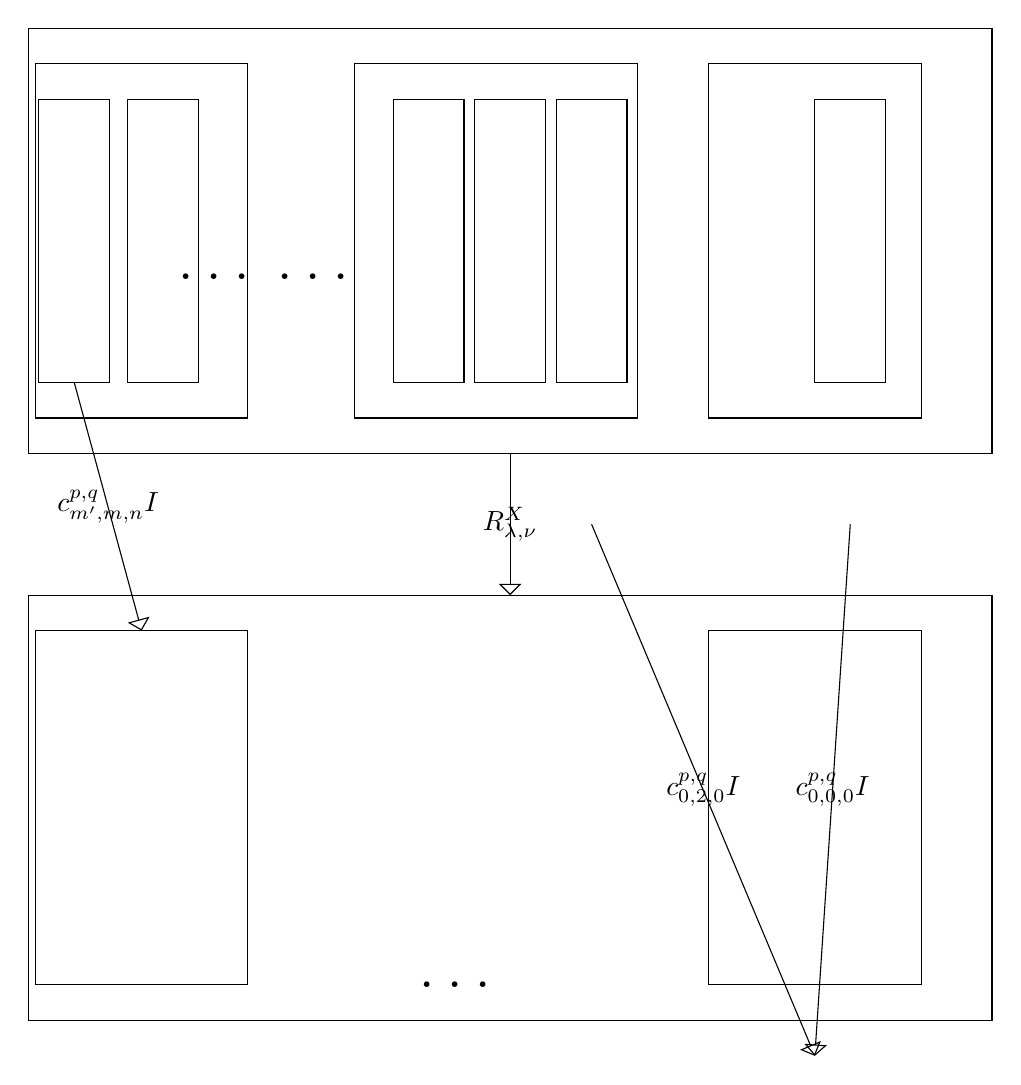
\begin{tikzpicture}[rotate=-90,scale=1.8]
	\draw[color=black] (-9.0,0.75) rectangle (-6.0,-6.05);%upper
\draw[color=black] (-8.75,0.25) rectangle (-6.25,-1.25);%right in upper
\draw[color=black] (-8.5,0.0) rectangle (-6.5,-0.5);%in ``right in upper''
\draw[color=black] (-8.75,-1.75) rectangle (-6.25,-3.75);%middle in upper
\draw[color=black] (-8.5,-1.825) rectangle (-6.5,-2.325);%right in ``middle in upper''
\draw[color=black] (-8.5,-2.4) rectangle (-6.5,-2.9);%middle in ``middle in upper''
\draw[color=black] (-8.5,-2.975) rectangle (-6.5,-3.475);%left in ``middle in upper''
\draw[color=black] (-8.75,-4.5) rectangle (-6.25,-6.0);%left in upper
\draw[color=black] (-8.5,-4.85) rectangle (-6.5,-5.35);%right in ``left in upper''
\draw[color=black] (-8.5,-5.475) rectangle (-6.5,-5.975); %left in ``left in upper''

\draw[color=black] (-5.0,0.75) rectangle (-2.0,-6.05);%lower
\draw[color=black] (-4.75,0.25) rectangle (-2.25,-1.25);%right in lower
\draw[color=black] (-4.75,-4.5) rectangle (-2.25,-6.0);%left in lower

\node at (-7.25,-4.0) {\color{black}{\Huge \dots}};
\node at (-7.25,-4.7) {\color{black}{\Huge \dots}};
\node at (-2.25,-3.0) {\color{black}{\Huge \dots}};

%%\node at (-7.0,1.0) {\color{black}{$I(\lambda)$}};
%%\node at (-2.0,1.0) {\color{black}{$J(\nu)$}};

\draw[-open triangle 90] (-6.0,-2.65) to node {$R_{\lambda,\nu}^X$} (-5.0,-2.65);
\draw[-open triangle 90] (-5.5,-0.25) to node {$c^{p,q}_{0,0,0}I$} (-1.75,-0.5);
\draw[-open triangle 90] (-5.5,-2.075) to node {$c^{p,q}_{0,2,0}I$} (-1.75,-0.5);
\draw[-open triangle 90] (-6.5,-5.725) to node {$c^{p,q}_{m',m,n}I$} (-4.75,-5.25);

	\end{tikzpicture}
	\caption{対称性破れ作用素と$(K,K')$タイプ}
	\label{fig:1}
\end{figure}
		\item $(K,K')$固有値がゼロになるかどうかを判定したい;
		\item $\mysbo$の積分核が別の手法で決定されたとする;
		\item 積分核を用いて、$(K,K')$固有値を積分の形で表示できる;
	\end{enumerate}
	群$(G,G')=(O(p+1,q),O(p,q))$に対する対称性破れ作用素の研究
	で命題\ref{prop:int-st-gg}
	の積分が{現}れた。命題\ref{prop:int-st-gg}では積分値
	がガンマ関数の積公式として与えられるのでゼロかどうかが完全に決定できる。

	\nocite{Selberg:411367}
	\nocite{warnaar2010sl3}
	\nocite{dotsenko1985four}
	\nocite{tarasov2003selberg}

%%	\bibliographystyle{alpha}
%%	\bibliography{intdep}
	\begin{thebibliography}{CK{\O}P11}
\expandafter\ifx\csname urlstyle\endcsname\relax
  \providecommand{\doi}[1]{doi:\discretionary{}{}{}#1}\else
  \providecommand{\doi}{doi:\discretionary{}{}{}\begingroup
  \urlstyle{rm}\Url}\fi

\bibitem[BR04]{bernstein2004estimates}
J.~Bernstein and A.~Reznikov.
\newblock Estimates of automorphic functions.
\newblock \emph{Mosc. Math. J}, \textbf{\textbf{4}}(1), (2004), pp. 19--37.
Available at \url{http://mi.mathnet.ru/eng/mmj141}.

\bibitem[CK{\O}P11]{clerc2011generalized}
J.-L. Clerc, T.~Kobayashi, B.~{\O}rsted and M.~Pevzner.
\newblock Generalized {B}ernstein--{R}eznikov integrals.
\newblock \emph{Math. Ann.}, \textbf{349}(2), (2011), pp. 395--431.
Available at \url{https://doi.org/10.1007/s00208-010-0516-4}.

\bibitem[HT93]{howe1993homogeneous}
R.~E. Howe and E.-C. Tan.
\newblock Homogeneous functions on light cones: the infinitesimal structure of
  some degenerate principal series representations.
\newblock \emph{Bull. Amer. Math. Soc.}, \textbf{28}(1), (1993), pp. 1--74.
Available at \url{http://www.ams.org/journals/bull/1993-28-01/S0273-0979-1993-00360-4/S0273-0979-1993-00360-4.pdf}.

\bibitem[J09]{juhl2009families}
A.~Juhl.
\newblock \emph{Families of {C}onformally {C}ovariant {D}ifferential
  {O}perators, {Q}-curvature and {H}olography}, \emph{Progr. Math,}
  \textbf{275}.
\newblock Springer Science \& Business Media (2009).
Available at \url{http://www.springer.com/in/book/9783764398996}.

\bibitem[K15]{kobayashi2015program}
T.~Kobayashi.
\newblock A program for branching problems in the representation theory of real
  reductive groups.
\newblock \emph{Progr. Math.}, \textbf{312}, (2015), pp. 277--322.
\newblock In: \emph{{\normalfont Special issue in honor of Vogan's 60th years
  birthday}}.
Available at \url{https://doi.org/10.1007/978-3-319-23443-4_10}.

\bibitem[K{\O}03]{KO2}
T.~Kobayashi and B.~{\O}rsted.
\newblock Analysis on the minimal representation of\/ {$\mbox{\rm O}(p,q)$}.{$\;$}{{\rm{II}}}. {B}ranching laws.
\newblock \emph{Adv. Math.}, \textbf{180}(2), (2003), pp. 513--550.
Available at \url{https://doi.org/10.1016/S0001-8708(03)00013-6}.

\bibitem[KO13]{kobayashi2013finite}
T.~Kobayashi and T.~Oshima.
\newblock Finite multiplicity theorems for induction and restriction.
\newblock \emph{Adv. Math.}, \textbf{248}, (2013), pp. 921--944.
Available at \url{http://dx.doi.org/10.1016/j.aim.2013.07.015}.

\bibitem[K93]{kobayashi1993}
T.~Kobayashi.
\newblock The restriction of ${A}_q \left( \lambda \right)$ to reductive
  subgroups.
\newblock \emph{Proc. Japan Acad. Ser. A Math. Sci.}, \textbf{69}(7), (1993),
  pp. 262--267.
Available at \url{http://dx.doi.org/10.3792/pjaa.69.262}.

\bibitem[K98]{10.2307/120963}
T.~Kobayashi.
\newblock Discrete decomposability of the restriction of ${A}_q(\lambda)$ with
  respect to reductive subgroups {I}{I}: Micro-local analysis and asymptotic
  {K}-support.
\newblock \emph{Annals of Mathematics}, \textbf{147}(3), (1998), pp. 709--729.
Available at \url{http://dx.doi.org/10.2307/120963}.

\bibitem[K14]{KOBAYASHI2014272}
T.~Kobayashi.
\newblock F-method for symmetry breaking operators.
\newblock \emph{Differential Geometry and its Applications}, \textbf{33},
  (2014), pp. 272 -- 289.
Available at \url{http://dx.doi.org/10.1016/j.difgeo.2013.10.003}.

\bibitem[K16]{kobayashi16birth}
T.~Kobayashi.
\newblock \emph{Birth of new branching problems}.
\newblock
  日本数学会70年記念 総合講演・企業特別講演アブストラクト, pp. 65--92,
  日本数学会, 2016.
Available at \url{http://www.ms.u-tokyo.ac.jp/~toshi/texpdf/tk2016p-msj70.pdf}.

\bibitem[K{\O}SS15]{kobayashi2015branching}
T.~Kobayashi, B.~{\O}rsted, P.~Somberg and V.~Sou{\v{c}}ek.
\newblock Branching laws for verma modules and applications in parabolic
  geometry. {I}.
\newblock \emph{Adv. Math.}, \textbf{285}, (2015), pp. 1796--1852.
Available at \url{http://dx.doi.org/10.1016/j.aim.2015.08.020}.

\bibitem[KP16a]{kobayashi2016differential1}
T.~Kobayashi and M.~Pevzner.
\newblock Differential symmetry breaking operators: I. {G}eneral theory and
  {F}-method.
\newblock \emph{Selecta Mathematica}, \textbf{22}(2), (2016), pp. 801--845.
Available at \url{http://dx.doi.org/10.1007/s00029-015-0207-9}.

\bibitem[KP16b]{Kobayashi2016}
T.~Kobayashi and M.~Pevzner.
\newblock Differential symmetry breaking operators: {I}{I}. {R}ankin--{C}ohen
  operators for symmetric pairs.
\newblock \emph{Selecta Mathematica}, \textbf{22}(2), (2016), pp. 847--911.
Available at \url{http://dx.doi.org/10.1007/s00029-015-0208-8}.

\bibitem[KS15]{kobayashi2015symmetry}
T.~Kobayashi and B.~Speh.
\newblock \emph{Symmetry {B}reaking for {R}epresentations of {R}ank {O}ne
  {O}rthogonal {G}roups}, \emph{Memoirs of the Amer. Math. Soc,} \textbf{238}.
\newblock American Mathematical Society (2015).
Available at \url{http://dx.doi.org/10.1090/memo/1126}.

\end{thebibliography}


\end{document}
